\documentclass{beamer}

\mode<presentation>{
	%\usetheme{CambridgeUS}
	%\usecolortheme{seahorse}
	\usetheme{Boadilla}
	\usecolortheme{beaver}
	\setbeamertemplate{navigation symbols}{}
}

\usepackage{graphicx}
\usepackage{booktabs}
\usepackage{algpseudocode}
\usepackage{hyperref}
\usepackage{tikz}
\usepackage[utf8]{inputenc}
\usepackage{listings}
\usepackage[export]{adjustbox}
\usepackage{aeguill}
\usepackage{amsmath}

%\setbeamertemplate{title page}[default][rounded=false]

\setbeamertemplate{title page}
{
%\vbox{}
\begingroup
\centering
\begin{beamercolorbox}[sep=8pt,center]{institute}
\usebeamerfont{institute}\insertinstitute
\end{beamercolorbox}
\vskip1em%
\begin{beamercolorbox}[sep=8pt,center]{title}
\usebeamerfont{title}\inserttitle\par%
\ifx\insertsubtitle\@empty%
\else%
\vskip0.25em%
{\usebeamerfont{subtitle}\usebeamercolor[fg]{subtitle}\insertsubtitle\par}%
\fi%
\end{beamercolorbox}%
\vfill
\begin{beamercolorbox}[sep=8pt,center]{author}
\usebeamerfont{author}\insertauthor
\end{beamercolorbox}
\vskip1em\par
\begin{beamercolorbox}[sep=8pt,center]{date}
\usebeamerfont{date}\insertdate
\end{beamercolorbox}
\endgroup
}

\setbeamertemplate{blocks}[default]
\setbeamercolor{structure}{fg=darkred}
%\setbeamercolor{block title}{bg=darkred,fg=white}
%\setbeamercolor{block body}{bg=darkgray!20!white}
\setbeamercolor{block title}{bg=darkgray!30!white}
\setbeamertemplate{enumerate items}[default]

\setbeamertemplate{part page}{
\begin{beamercolorbox}[sep=8pt,center,wd=\textwidth]{part title}
\usebeamerfont{part title}\insertpart\par
\end{beamercolorbox}
\vfill
\tableofcontents
}

%\setbeamertemplate{frametitle continuation}{(\insertcontinuationcount)}

\setbeamertemplate{headline}{\leavevmode\hbox{\begin{beamercolorbox}[wd=.5\paperwidth,ht=2.65ex,dp=1.5ex,center]{section in head/foot}\usebeamerfont{section in head/foot}\insertsectionhead\hspace*{2ex}
\end{beamercolorbox}\begin{beamercolorbox}[wd=.5\paperwidth,ht=2.65ex,dp=1.5ex,center]{subsection in head/foot}\usebeamerfont{subsection in head/foot}\hspace*{2ex}\insertsubsectionhead\end{beamercolorbox}}\vskip0pt}

\newcommand{\tcc}[1]{\textcolor{darkred}{#1}}

\newcommand{\codeA}[1]{\texttt{#1}}
\newcommand{\codeB}[1]{\texttt{\textcolor{darkred}{#1}}}

\newcommand{\link}[1]{{\footnotesize » \url{#1}}}
\newcommand{\bothquote}[1]{``#1''}

\definecolor{mygreen}{rgb}{0,0.6,0}
\definecolor{mygray}{rgb}{0.5,0.5,0.5}
\definecolor{mymauve}{rgb}{0.58,0,0.82}
\definecolor{maroon}{rgb}{0.5,0,0}
\definecolor{darkgreen}{rgb}{0,0.5,0}

\lstdefinelanguage{XML}
{
  basicstyle=\scriptsize\ttfamily,
  morestring=[s]{"}{"},
  morecomment=[s]{?}{?},
  morecomment=[s]{!--}{--},
  commentstyle=\color{darkgreen},
  moredelim=[s][\color{black}]{>}{<},
  moredelim=[s][\color{red}]{\ }{=},
  stringstyle=\color{blue},
  identifierstyle=\color{maroon},
  numbers=none
}

\lstdefinelanguage{Scala}{
  morekeywords={%
          abstract,case,catch,class,def,do,else,extends,%
          false,final,finally,for,forSome,if,implicit,import,lazy,%
          match,new,null,object,override,package,private,protected,%
          return,sealed,super,this,throw,trait,true,try,type,%
          val,var,while,with,yield},
  otherkeywords={=>,<-,<\%,<:,>:,\#,@},
  sensitive=true,
  morecomment=[l]{//},
  morecomment=[n]{/*}{*/},
  morestring=[b]",
  morestring=[b]',
  morestring=[b]"""
}[keywords,comments,strings]

\lstset{
    language=Scala,
    basicstyle=\scriptsize\ttfamily,
    keywordstyle=\scriptsize\color{blue}\ttfamily,
    commentstyle=\scriptsize\color{mygreen}\ttfamily,
    breakatwhitespace=false,
    breaklines=true,
    numbers=left,
      numberstyle=\color{mymauve},
      stringstyle=\color{mymauve},
      showstringspaces=false,
      numbers=none
}

\lstdefinestyle{floating}{%
    xleftmargin=10pt,%
    xrightmargin=5pt,%
    aboveskip=4mm,%
    belowskip=4mm,%
    fontadjust=true,%
    columns=[c]flexible,%
    keepspaces=true,%
    basewidth={0.5em, 0.425em},%
    tabsize=2,%
    basicstyle=\renewcommand{\baselinestretch}{0.95}\ttfamily,%
    commentstyle=\rm,%
    keywordstyle=\bfseries,%
    mathescape=true,%
    captionpos=b,%
    framerule=0.3pt,%
    firstnumber=0,%
    numbersep=1.5mm,%
    numberstyle=\tiny,%
    float=tbp,%
    frame=tblr,%
    framesep=5pt,%
    framexleftmargin=3pt,%
    abovecaptionskip=\smallskipamount,%
    belowcaptionskip=\smallskipamount,%
} % to define: caption, label

\makeatother

\AtBeginSection[]
{
  \begin{frame}
    \frametitle{Outline}
    \tableofcontents[currentsection]
  \end{frame}
}

%\AtBeginSubsection[]
%{
%  \begin{frame}
%    \frametitle{Outline}
%    \tableofcontents[currentsection,currentsubsection]
%  \end{frame}
%}

\institute[UNIBO]{\uppercase{Alma Mater Studiorum -- Università di Bologna}\\Dipartimento di Informatica -- Scienza e Ingegneria (DISI)\\C.d.S. in Ingegneria e Scienze Informatiche, Campus di Cesena}

\author[A. Marfoglia]{Alberto Marfoglia\\\scriptsize\texttt{alberto.marfoglia@studio.unibo.it}}

\title{ZIO}
\subtitle{componibilità e type safety a supporto della programmazione concorrente e asincrona}

\begin{document}

\begin{frame}
  \maketitle
\end{frame}

\begin{frame}{Piano di presentazione}
    \tableofcontents 
\end{frame}

\section{Introduzione}
\begin{frame}{Cos'è ZIO?}
  \begin{columns}
    \begin{column}{.5\textwidth}
      \begin{figure}
        \centering
        
\includegraphics[width=0.9\textwidth]{img/zio-logo.jpg}
        \label{ZIO logo.}
      \end{figure}
    \end{column}
    \begin{column}{.5\textwidth}
      \begin{center} 
        \texttt{ZIO} è una libreria puramente funzionale, \texttt{type-safe}, e componibile a supporto della programmazione concorrente e asincrona in Scala.
      \end{center}
    \end{column}
  \end{columns}
\end{frame}
%
\begin{frame}
    \frametitle{Perchè ZIO?}
    \begin{columns}
        \begin{column}{.5\textwidth}
            \centering{\small
              {\textbf{Concorrenza}}\break
              applicazioni concorrenti esenti da \textit{deadlocks} e \textit{race conditions}.
            }
        \end{column}
        \begin{column}{.5\textwidth}
            \centering{\small
              {\textbf{Efficienza}}\break
              cancellazione automatica di computazioni non più necessarie.
            }
        \end{column}
    \end{columns}
    
    \bigskip

    \begin{columns}
      \begin{column}{.5\textwidth}
          \centering{\small
            {\textbf{Resource-safety}}\break
            gestione automatica del ciclo di vita delle risorse.
          }
      \end{column}
      \begin{column}{.5\textwidth}
        \centering{\small
          {\textbf{Resilienza}}\break
          gestione statica degli errori, \texttt{Error channel} e meccanismi di \textit{scheduling}.
        }
      \end{column}
    \end{columns}

    \bigskip

    \begin{columns}
      \begin{column}{.5\textwidth}
          \centering{\small
            {\textbf{Testkit}}\break
            sviluppo rapido di test deterministici e \textit{type-safe}.
          }
      \end{column}
      \begin{column}{.5\textwidth}
        \centering{\small
          {\textbf{Streaming}}\break
          presenza di \textit{stream} efficienti, \textit{lazy}, \textit{resource-safe}, concorrenti e infiniti.
        }
      \end{column}
    \end{columns}
        
\end{frame}
\section{Elementi fondamentali}

\begin{frame}{Functional Effects}
  \begin{block}{\textit{Purely functional programming}}
    \texttt{ZIO} permette di sviluppare codice puramente funzionale, cioè i programmi possono essere descritto come composizione di espressioni che rispettano le seguenti proprietà: 
    \begin{itemize}
      \item \textbf{\textit{referential transparency}}: le espressioni sono sostituibili dai valori;
      \item \textbf{\textit{local reasoning}}: le funzioni sono autoesplicative.
    \end{itemize}
    Queste facilitano il \textit{refactoring} e la comprensione del codice.
  \end{block}

  \begin{alertblock}{Perchè i \textit{side effect} sono un problema?}
    Le proprietà appena presentate vengono meno nel caso di \textit{side effects}. Serve quindi un ponte tra questi e la programmazione puramente funzionale.
  \end{alertblock}
\end{frame}

\begin{frame}{Functional Effects II}
  \begin{block}{ZIO Core}
    \vspace{4mm}
    \begin{columns}
      \begin{column}{.5\textwidth}
        Il tipo di dato principale di \texttt{ZIO} è \texttt{ZIO[-R, +E, +A]} che consente di convertire istruzioni in \textit{functional effect} al fine di ritardarne la valutazione.
      \end{column}
      \begin{column}{.4\textwidth}
        \begin{itemize}
          \item \texttt{R} - \textit{environment type}.
          \item \texttt{E} - \textit{error type}.
          \item \texttt{A} - \textit{success type}.
        \end{itemize}
      \end{column}
    \end{columns}
    \vspace{2mm}
  \end{block}

  \begin{exampleblock}{Vantaggi}
    \begin{itemize}
      \item Separazione tra il "cosa" il programma dovrà fare dal "come" lo farà.
      \item Sviluppo incrementale di programmi complessi tramite \textbf{componibilità}.
      \item Fruizione dei vantaggi del \textit{type system} di Scala. 
      %\lstinline[language=Scala]{ZIO[Clock, Nothing, Unit]}
    \end{itemize}
  \end{exampleblock}
\end{frame}

\begin{frame}[fragile]{ZIO Constructors \& Operators}
  \begin{block}{\texttt{ZIO} constructors}
    I costruttori di \texttt{ZIO} permetto di ricondurre codice affetto da \textit{side-effects} a funzioni pure componibili. Tra i principali:
    \begin{itemize}
      \item \texttt{ZIO.succeed}: converte valori puri;
      \item \texttt{ZIO.attempt}: converte codice procedurale affetto da \textit{side-effects};
      \item \texttt{ZIO.async}: converte codice asincrono basato su \textit{callbacks};
      \item \texttt{ZIO.fromFuture}: converte una funzione che crea una \texttt{Future}.
    \end{itemize}
  \end{block}
  \begin{block}{\texttt{ZIO} operators}
    Una peculiarità di \texttt{ZIO} sono gli operatori, come \texttt{flatMap}, \texttt{foreach}, \texttt{zip}, \texttt{collectAll}, che permettono di trasformare e combinare \textit{effect} tra loro.
    \begin{itemize}
      \item \small\texttt{flatMap} + \textit{for comprehension} 
      $\rightarrow$ espressività programmazione imperativa.
    \end{itemize}
  \end{block}
\end{frame}

\begin{frame}[fragile]{ZIO Constructors \& Operators II}
  \begin{block}{Esempio: assegnazione di un \textit{task}}
    \lstinputlisting[language=Scala]{code/1a-effects.scala}
  \end{block}
  \pause
  \begin{block}{Esempio: assegnazione di un \textit{task} in \texttt{ZIO}}
    \lstinputlisting[language=Scala]{code/1b-effects.scala}
  \end{block}
\end{frame}


\section{ZIO Error Model}

\begin{frame}{Gestione degli errori in \texttt{ZIO}}

  \begin{block}{Tipologie di fallimento}
    \texttt{ZIO} definisce tre possibili tipologie di fallimento:
    \begin{itemize}
      \item \textbf{\textit{Failures}}: modellano scenari di fallimento prevedibili (\textit{error type}).
      \item \textbf{\textit{Defects}}: modellano errori imprevedibili (convertibili in \textit{failures}).
      \item \textbf{\textit{Fatals}}: errori catastrofici che causano la terminazione del programma.
    \end{itemize}
  \end{block}

  \begin{block}{Gestione dichiarativa degli errori}
    In un approccio dichiarativo, gli errori vengono rappresentati come valori.
    \begin{itemize}
      \item \textit{referential transparency}: non è necessario interrompere il flusso; 
      \item \textit{exhaustive checking}: gli errori sono tipi di dato chiuso;
      \item \textit{type safety}: previene la scrittura di codice \textit{unsafe};
      \item \textit{error model}: modello \texttt{Cause[+E]} più espressivo di \texttt{try/catch}.
    \end{itemize}
  \end{block}
\end{frame}

\begin{frame}
  \begin{block}{Gestione delle \textit{Failure}}
    \begin{itemize}
      \item Una \textit{failure} può essere modellata tramite il costruttore \texttt{ZIO.fail}.
      \item Le \textit{failure} possono essere recuperate tramite l'operatore \texttt{catchAll}.
      \item Le \textit{failure} possono diventare \textit{defect} tramite l'operatore \texttt{orDie}.
    \end{itemize}
  \end{block}

  \begin{block}{Esempio: recupero di una \textit{Failure}}
    \lstinputlisting[language=Scala]{code/1c-error-match.scala}
  \end{block}
\end{frame}
\section{Parallelismo e Concorrenza}

\begin{frame}[fragile]{Il Modello Fiber}

  \begin{columns}
    \begin{column}{.6\textwidth}
      \begin{figure}
        \centering
            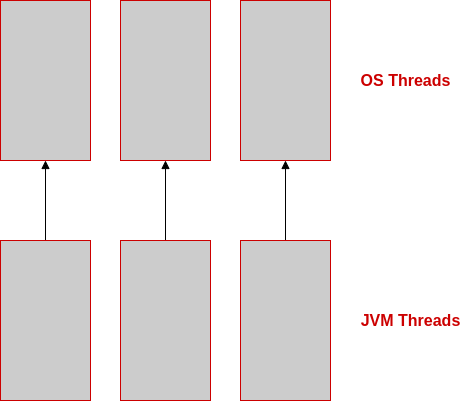
\includegraphics[width=0.9\textwidth]{img/jvm-threads.png}
            \label{JVM threads mapping.}
        \end{figure}
    \end{column}
    \begin{column}{.35\textwidth}
      \begin{block}{\centering Thread massimi}
        \vspace{2mm}
        \centering{\Large{10.000}}
        \vspace{2mm}
      \end{block}
      \vspace{4.5mm}
      \begin{block}{Dificoltà a scalare}
        \begin{itemize}
          \item \textit{shutdown esplicito}
          \item \textit{context switching}
          \item \textit{stack preallocato}
        \end{itemize}
      \end{block}
    \end{column}
  \end{columns}

\end{frame}

\begin{frame}[fragile]{Il Modello Fiber II}

  \begin{columns}
    \begin{column}{.6\textwidth}
      \begin{figure}
        \centering
            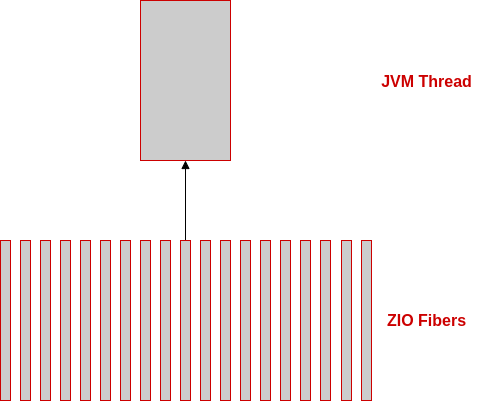
\includegraphics[width=0.9\textwidth]{img/fibers.png}
            \label{Fibers mapping.}
        \end{figure}
    \end{column}
    \begin{column}{.35\textwidth}
      \begin{block}{\centering Fiber massime}
        \vspace{2mm}
        \centering{\Large{1.000.000}}
        \vspace{2mm}
      \end{block}
      \vspace{4.5mm}
      \begin{block}{Elevata scalabilità}
        \begin{itemize}
          \item tipo componibile
          \item \textit{garbage collected}
          \item tempo di CS ridotto
          \item \textit{stack} dinamico
          \item supervisione
        \end{itemize}
      \end{block}
    \end{column}
  \end{columns}

\end{frame}

\begin{frame}{Interruzione}
  \begin{block}{ZIO Runtime}
    Nel caso in cui un \textit{effect} fosse seguito da un'interruzione e il suo risultato fosse inutilizzato, il \textit{runtime} di \texttt{ZIO} può decidere di non eseguirlo:
    \begin{itemize}
      \item ogni parte di un \textit{effect} può essere interrompibile
      \begin{itemize}
        \item fanno eccezione blocchi di codice importato affetti da \textit{side effect};
      \end{itemize}
      \item l'interruzione attende l'esecuzione di eventuali \textit{finalizer} (\texttt{ensuring});
    \end{itemize}
  \end{block}
  \begin{block}{Esempio: semplice interruzione}
    \lstinputlisting[language=Scala]{code/4a-interruzione.scala}    
  \end{block}
\end{frame}

\begin{frame}{Strutture Concorrenti}
  \begin{block}{Ref - Condivisione di stato}
    Per permette a più \textit{fiber} di condividere informazioni, \texttt{ZIO} fornisce la struttura \texttt{Ref}. Questa descrive una modifica di stato:
    \begin{itemize}
      \item alternativa puramente funzionale dell'\texttt{AtomicReference};
      \item le operazioni di accesso e modifica sono atomiche (\textit{safe}).
    \end{itemize}
  \end{block}
  \begin{block}{Esempio: modellazione di un contatore}
    \lstinputlisting[language=Scala]{code/4b-contatore.scala}    
  \end{block}
\end{frame}

\begin{frame}{Strutture Concorrenti II}
  \begin{block}{Queue - Distribuzione del lavoro}
    Una \texttt{Queue} consente di gestire molteplici valori distribuibili tra più \textit{fiber}.
     \begin{itemize}
      \item le operazioni fondamentali sono \texttt{offer} e \texttt{take};
      \item le possibili tipologie sono \texttt{unbounded} e \texttt{bounded};
      \item le strategie di inserimento sono \textit{Back pressure}, \textit{Sliding} e \textit{Dropping}.
     \end{itemize}
  \end{block}
  
  \begin{figure}
    \centering
    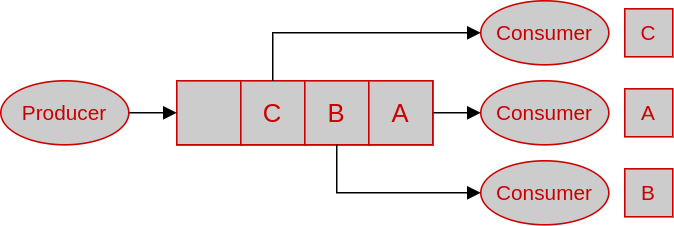
\includegraphics[width=0.7\textwidth]{img/queue.png}
    \label{distributing with queue.}
  \end{figure}

  % \begin{block}{Esempio: ping-pong con \texttt{bounded Queue}}
  %   \lstinputlisting[language=Scala]{code/4c-pingpong.scala}    
  % \end{block}

\end{frame}

\begin{frame}{Strutture Concorrenti III}
  \begin{block}{Hub - Broadcasting}
    La struttura \texttt{Hub} realizza un \textit{broadcasting} di informazioni:
    \begin{itemize}
      \item le operazioni fondamentali sono \texttt{publish} e \texttt{subscribe};
      \item le possibili tipologie sono \texttt{unbounded} e \texttt{bounded};
      \item le strategie di inserimento sono \textit{Back pressure}, \textit{Sliding} e \textit{Dropping}.
    \end{itemize}
  \end{block}
  \begin{figure}
    \centering
    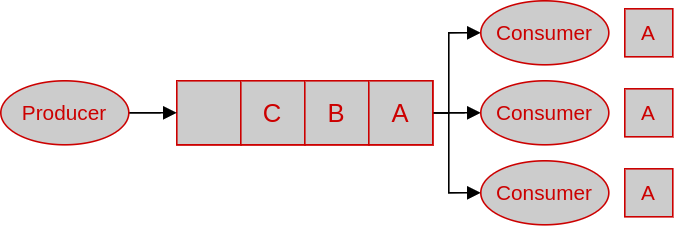
\includegraphics[width=0.7\textwidth]{img/hub.png}
    \label{broadcasting with hub.}
  \end{figure}
\end{frame}


\section{Dependency Injection}
\begin{frame}{}
  \begin{block}{Environment}
    \centering{
    \lstinline[language=Scala]{type ZIO[-R, +E, +A] = ZEnvironment[R] => Either[Cause[E], A]}
    }
    \vspace{2mm}
    \begin{itemize}
      \item \texttt{R} raccoglie un insieme di funzionalità valide localmente (\small{\textit{SRP}}).
      \item \texttt{R} può definire le dipendenze di un \textit{workflow}.
      \begin{itemize}
        \item in linea con architetture costruite a "strati" (\textit{Onion architecture} ).
      \end{itemize} 
    \end{itemize}
  \end{block}

  \begin{block}{ZLayer}
    Il tipo \texttt{ZLayer[RIn, E, ROut]} semplifica la costruzione degli "strati"
    \begin{itemize}
      \item componibile verticalmente e orizzontalmente
      \item controllo delle dipendenze mancanti a \textit{compile time}
      \item migliora la leggibilità del codice
      \item consente di aggiungere una logica di inizializzazione e di finalizzazione
    \end{itemize}

  \end{block}
  
\end{frame}

\begin{frame}{The Service Pattern}
  \begin{block}{Esempio: implementazione del Service Pattern}
    \lstinputlisting[language=Scala]{code/5a-service-pattern.scala}
  \end{block}
\end{frame}

\begin{frame}{The Service Pattern II}
  \begin{block}{}
    \lstinputlisting[language=Scala]{code/5b-service-pattern.scala}
  \end{block}
  \pause
  \begin{alertblock}{}
    \lstinputlisting[language=Scala]{code/5c-service-pattern.scala}
  \end{alertblock}
  \pause
  \begin{exampleblock}{}
    \lstinputlisting[language=Scala]{code/5d-service-pattern.scala}
  \end{exampleblock}
\end{frame}
\section{STM - Software Transactional Memory}
\begin{frame}{ZSTM}
  \begin{block}{Definizione}
    STM è uno strumento che permette di comporre singole operazioni in un'unica transazione eseguibile in maniera atomica. In \texttt{ZIO} viene rappresentato dalla struttura \texttt{ZSTM[R, E, A]}.
  \end{block}

  \begin{exampleblock}{Vantaggi}
    \begin{itemize}
      \item più potenti di \texttt{Ref}, poiché componibili
      \item esegue transazioni condizionali evitando l'utilizzo di \textit{locks}
      \item le transazioni sono libere da \textit{deadlocks} o \textit{race conditions}
    \end{itemize}
  \end{exampleblock}

  \begin{alertblock}{Limitazioni}
    \begin{itemize}
      \item non è possibile eseguire istruzioni concorrenti all'interno di una ZSTM
      \item nel caso di forte contesa vi è un calo di \textit{performance}
    \end{itemize}
  \end{alertblock}
\end{frame}

\begin{frame}{ZSTM II}
  \begin{block}{Esempio: trasferimento bancario}
    \lstinputlisting[language=Scala]{code/6a-zstm.scala}
  \end{block}
  \begin{block}{Operatori}
    \begin{itemize}
      \item \texttt{retry}: permette di rieseguire un'intera transazione
      \item \texttt{commit}: converte una transazione in uno \texttt{ZIO} \textit{effect}
    \end{itemize}
  \end{block}
\end{frame}
\section{Streaming con ZIO}
\begin{frame}{ZIO Stream}
  \begin{figure}
    \centering
    
\includegraphics[width=0.9\textwidth]{img/zio-stream.png}
    \label{ZIO logo.}
  \end{figure}
  \begin{block}{ZStream}
    \texttt{ZIO} implementa il paradigma \textit{streaming} attraverso il supporto \texttt{ZIO Stream}. Il tipo di dato principale è \texttt{ZStream[R, E, O]}:
    \begin{itemize}
      \item dichiarativo e di alto livello
      \item asincrono e scalabile
      \item efficiente (\textit{chunk}) e \textit{resource-safe}
      \item flusso di dati potenzialmente infinito
      \item concorrente e parallelizzabile
    \end{itemize}
  \end{block}
\end{frame}

\begin{frame}{ZIO Stream II}
    \begin{block}{Esempio: lettura di un file come uno \textit{stream} di linee}
    \lstinputlisting[language=Scala]{code/7a-stream.scala}    
  \end{block}
\end{frame}
\section{Conclusioni}
\begin{frame}{Conclusioni}

  \begin{columns}
    \begin{column}{.86\textwidth}
      \begin{block}{\centering Ecosistema}
        \vspace{2mm}
        \centering
      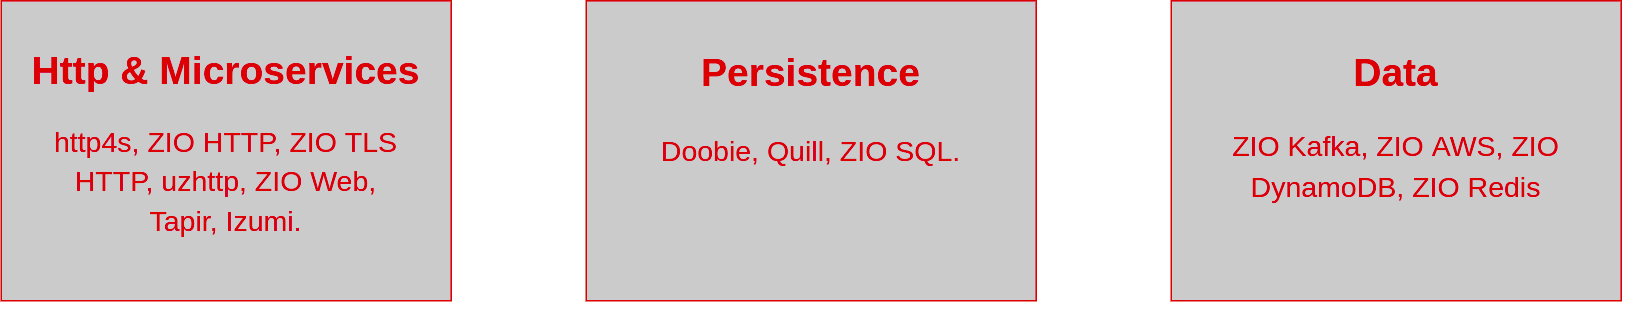
\includegraphics[width=0.9\textwidth]{img/zio-ecosystem.png}
      \label{ecosystem.}
      \end{block}
    \end{column}
  \end{columns}

  \begin{columns}
    \begin{column}{.25\textwidth}
      \begin{block}{\centering Download (2021)}
        \vspace{2mm}
        \centering{\large{$\backsimeq$ 1M}}
        \vspace{2mm}
      \end{block}
      \begin{block}{\centering Contributor}
        \begin{figure}
          \centering
          
\includegraphics[width=0.9\textwidth]{img/ziverge.png}
          \label{ziverge.}
        \end{figure}
      \end{block}
    \end{column}
    \begin{column}{.5\textwidth}
      \begin{figure}
        \centering
        
\includegraphics[width=1\textwidth]{img/companies.png}
        \label{companies adopted ZIO.}
      \end{figure}
    \end{column}
    
  \end{columns}
  
\end{frame}

%\begin{frame}{Bibliografia e siti web}

  \begin{thebibliography}{9}
      \setbeamertemplate{bibliography item}[book]
      \bibitem{} Zionomicon
      \newblock John De Goes, Adam Fraser 
      
      \setbeamertemplate{bibliography item}[online]
      \bibitem{} ZIO - dev
      \newblock \url{https://zio.dev/}
      
      \setbeamertemplate{bibliography item}[online]
      \bibitem{} ZIO catechism
      \newblock \url{https://zio.surge.sh/}
      
      \setbeamertemplate{bibliography item}[online]
      \bibitem{} ZIO - Resources
      \newblock \url{https://zio.dev/resources/}

      \setbeamertemplate{bibliography item}[online]
      \bibitem{} ZIO - Scala School
      \newblock \url{https://scala.school/}
  \end{thebibliography}
  
\end{frame}

\end{document}

